\documentclass[11pt]{book}

\input macros

\begin{document}
\mainmatter
%\input src/titlepage

\newpage

\thispagestyle{empty}
~
%\begin{tikzpicture}[overlay, remember picture]
  %\node[inner sep=0pt, minimum width=\paperwidth, minimum height=\paperheight] at (current page.center) {
    %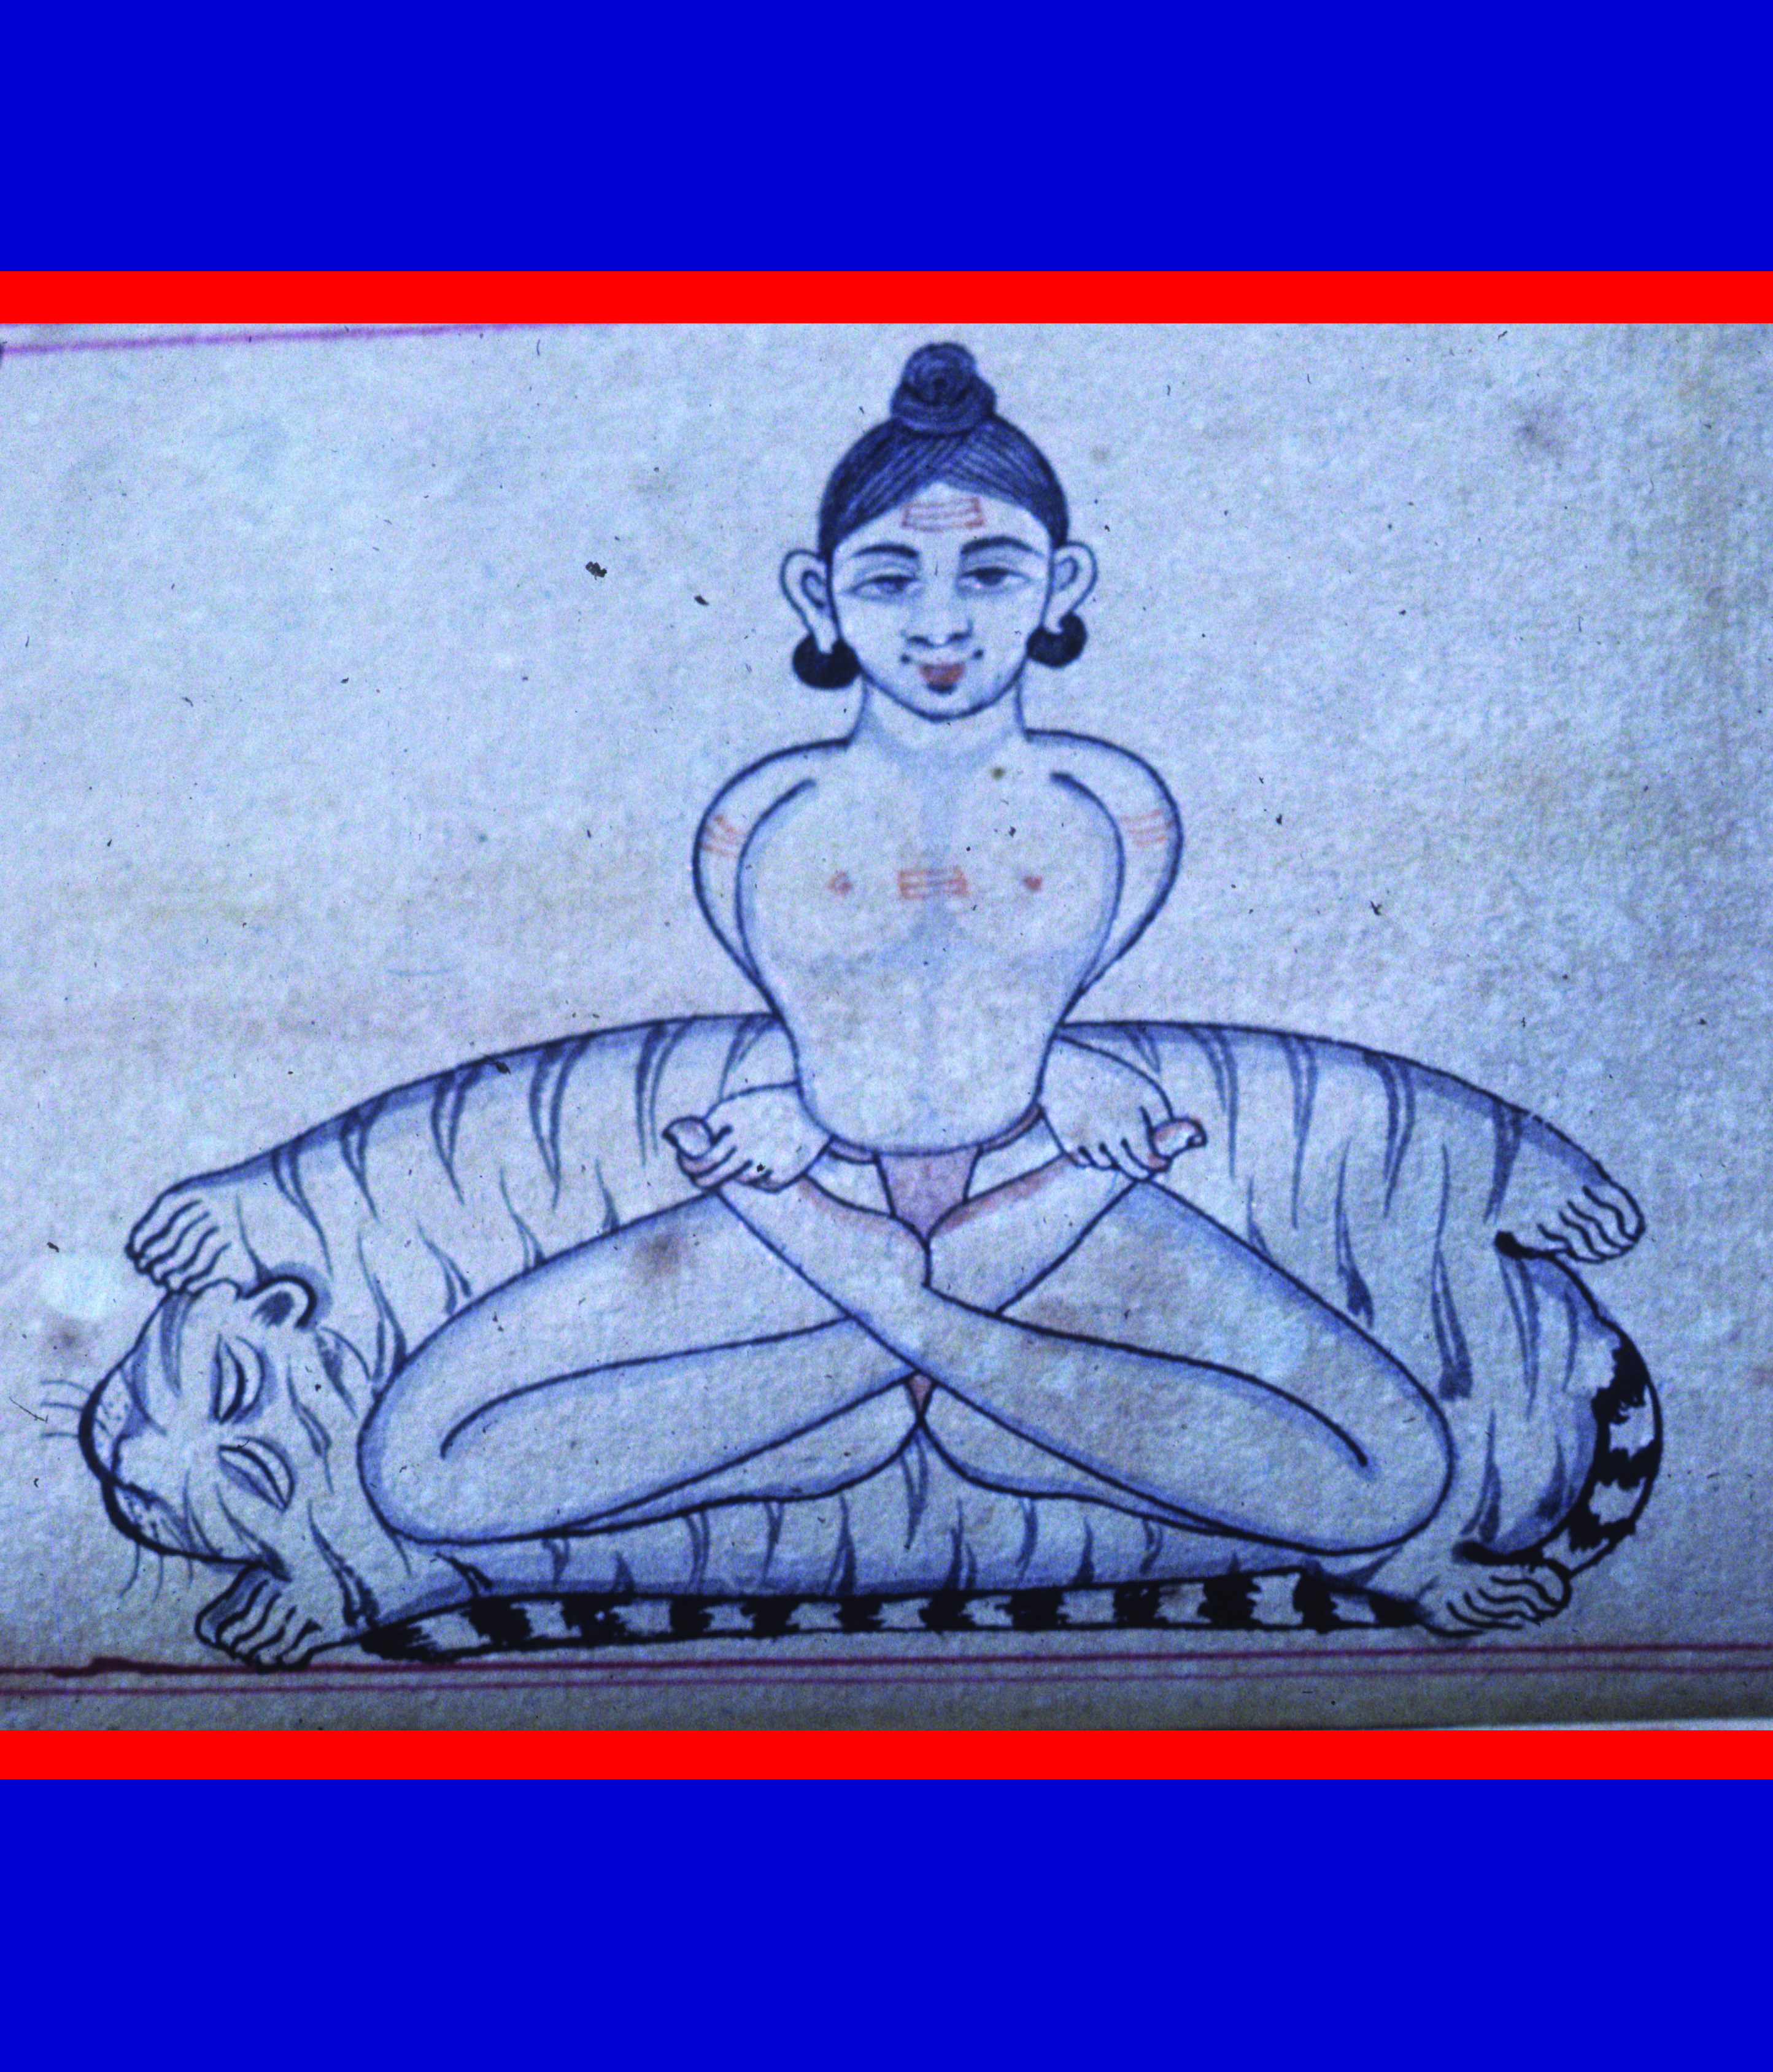
\includegraphics[width=\paperwidth, height=\paperheight, keepaspectratio]{1.jpg}
  %};
%\end{tikzpicture}

%\newpage

%\begin{tikzpicture}[overlay, remember picture]
  %\node[inner sep=0pt, minimum width=\paperwidth, minimum height=\paperheight] at (current page.center) {
    %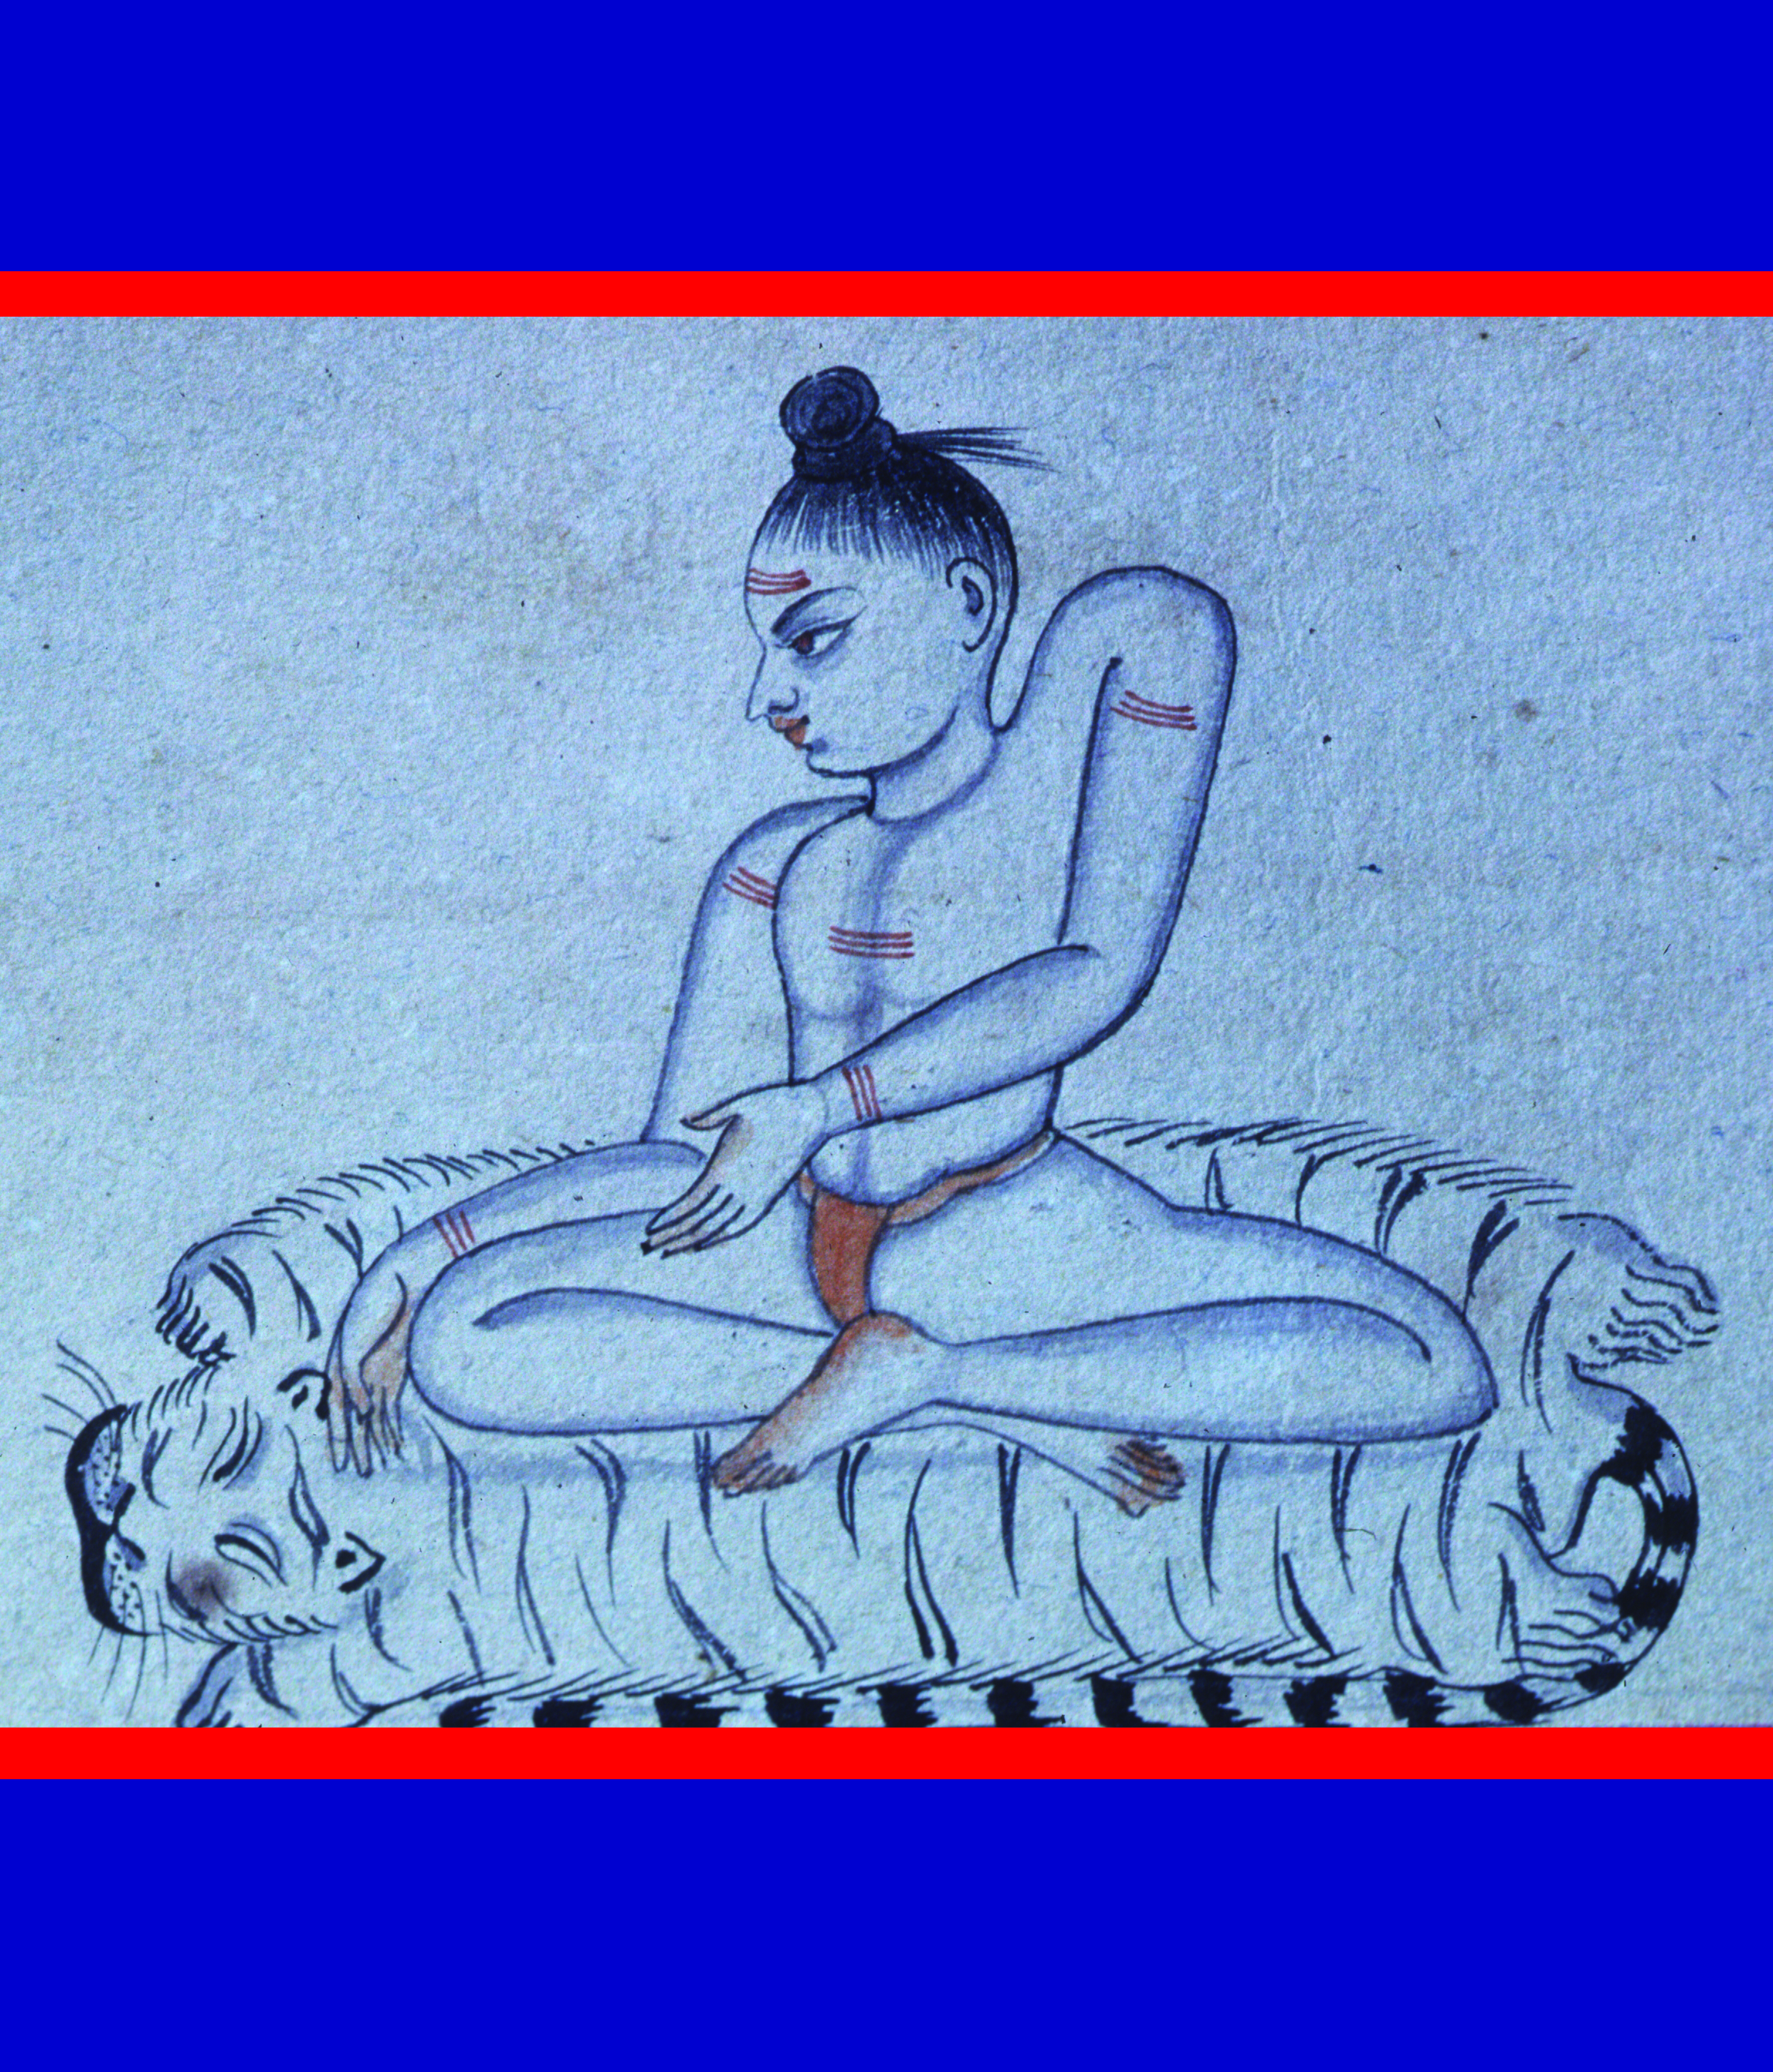
\includegraphics[width=\paperwidth, height=\paperheight, keepaspectratio]{2.jpg}
  %};
%\end{tikzpicture}

%\newpage

%\begin{tikzpicture}[overlay, remember picture]
  %\node[inner sep=0pt, minimum width=\paperwidth, minimum height=\paperheight] at (current page.center) {
    %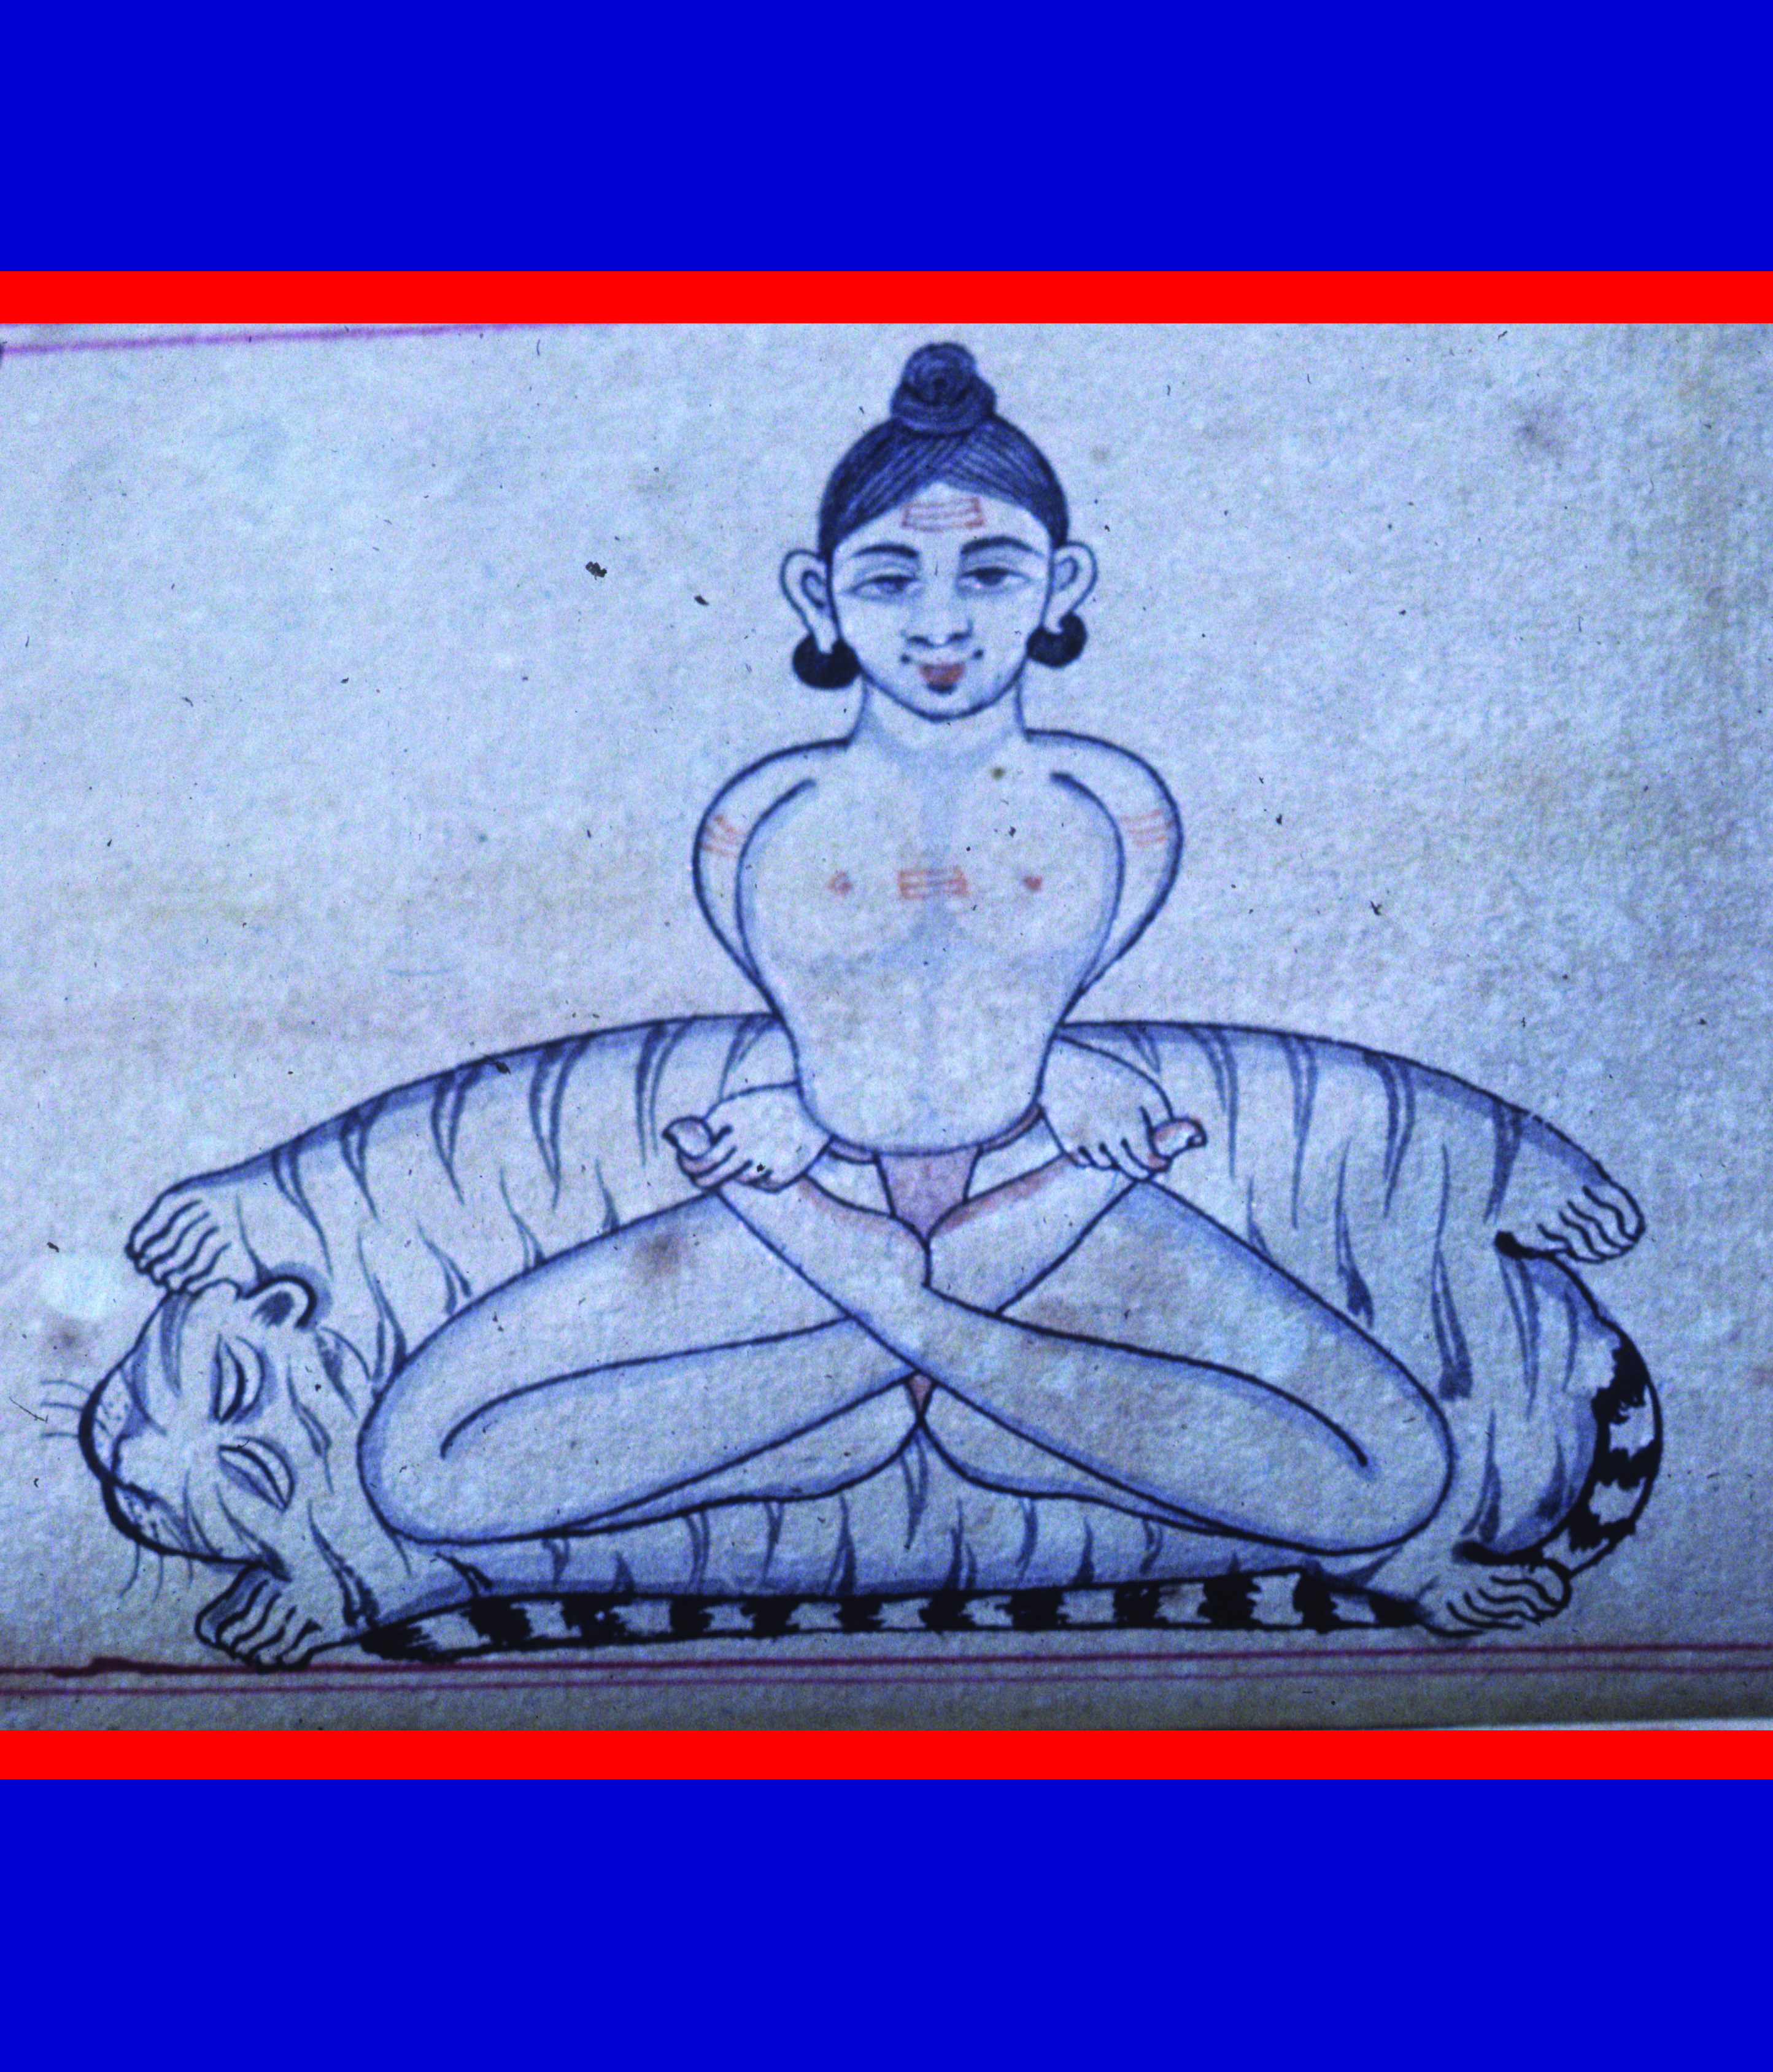
\includegraphics[width=\paperwidth, height=\paperheight, keepaspectratio]{1.jpg}
  %};
%\end{tikzpicture}

%\newpage

%\begin{tikzpicture}[overlay, remember picture]
  %\node[inner sep=0pt, minimum width=\paperwidth, minimum height=\paperheight] at (current page.center) {
    %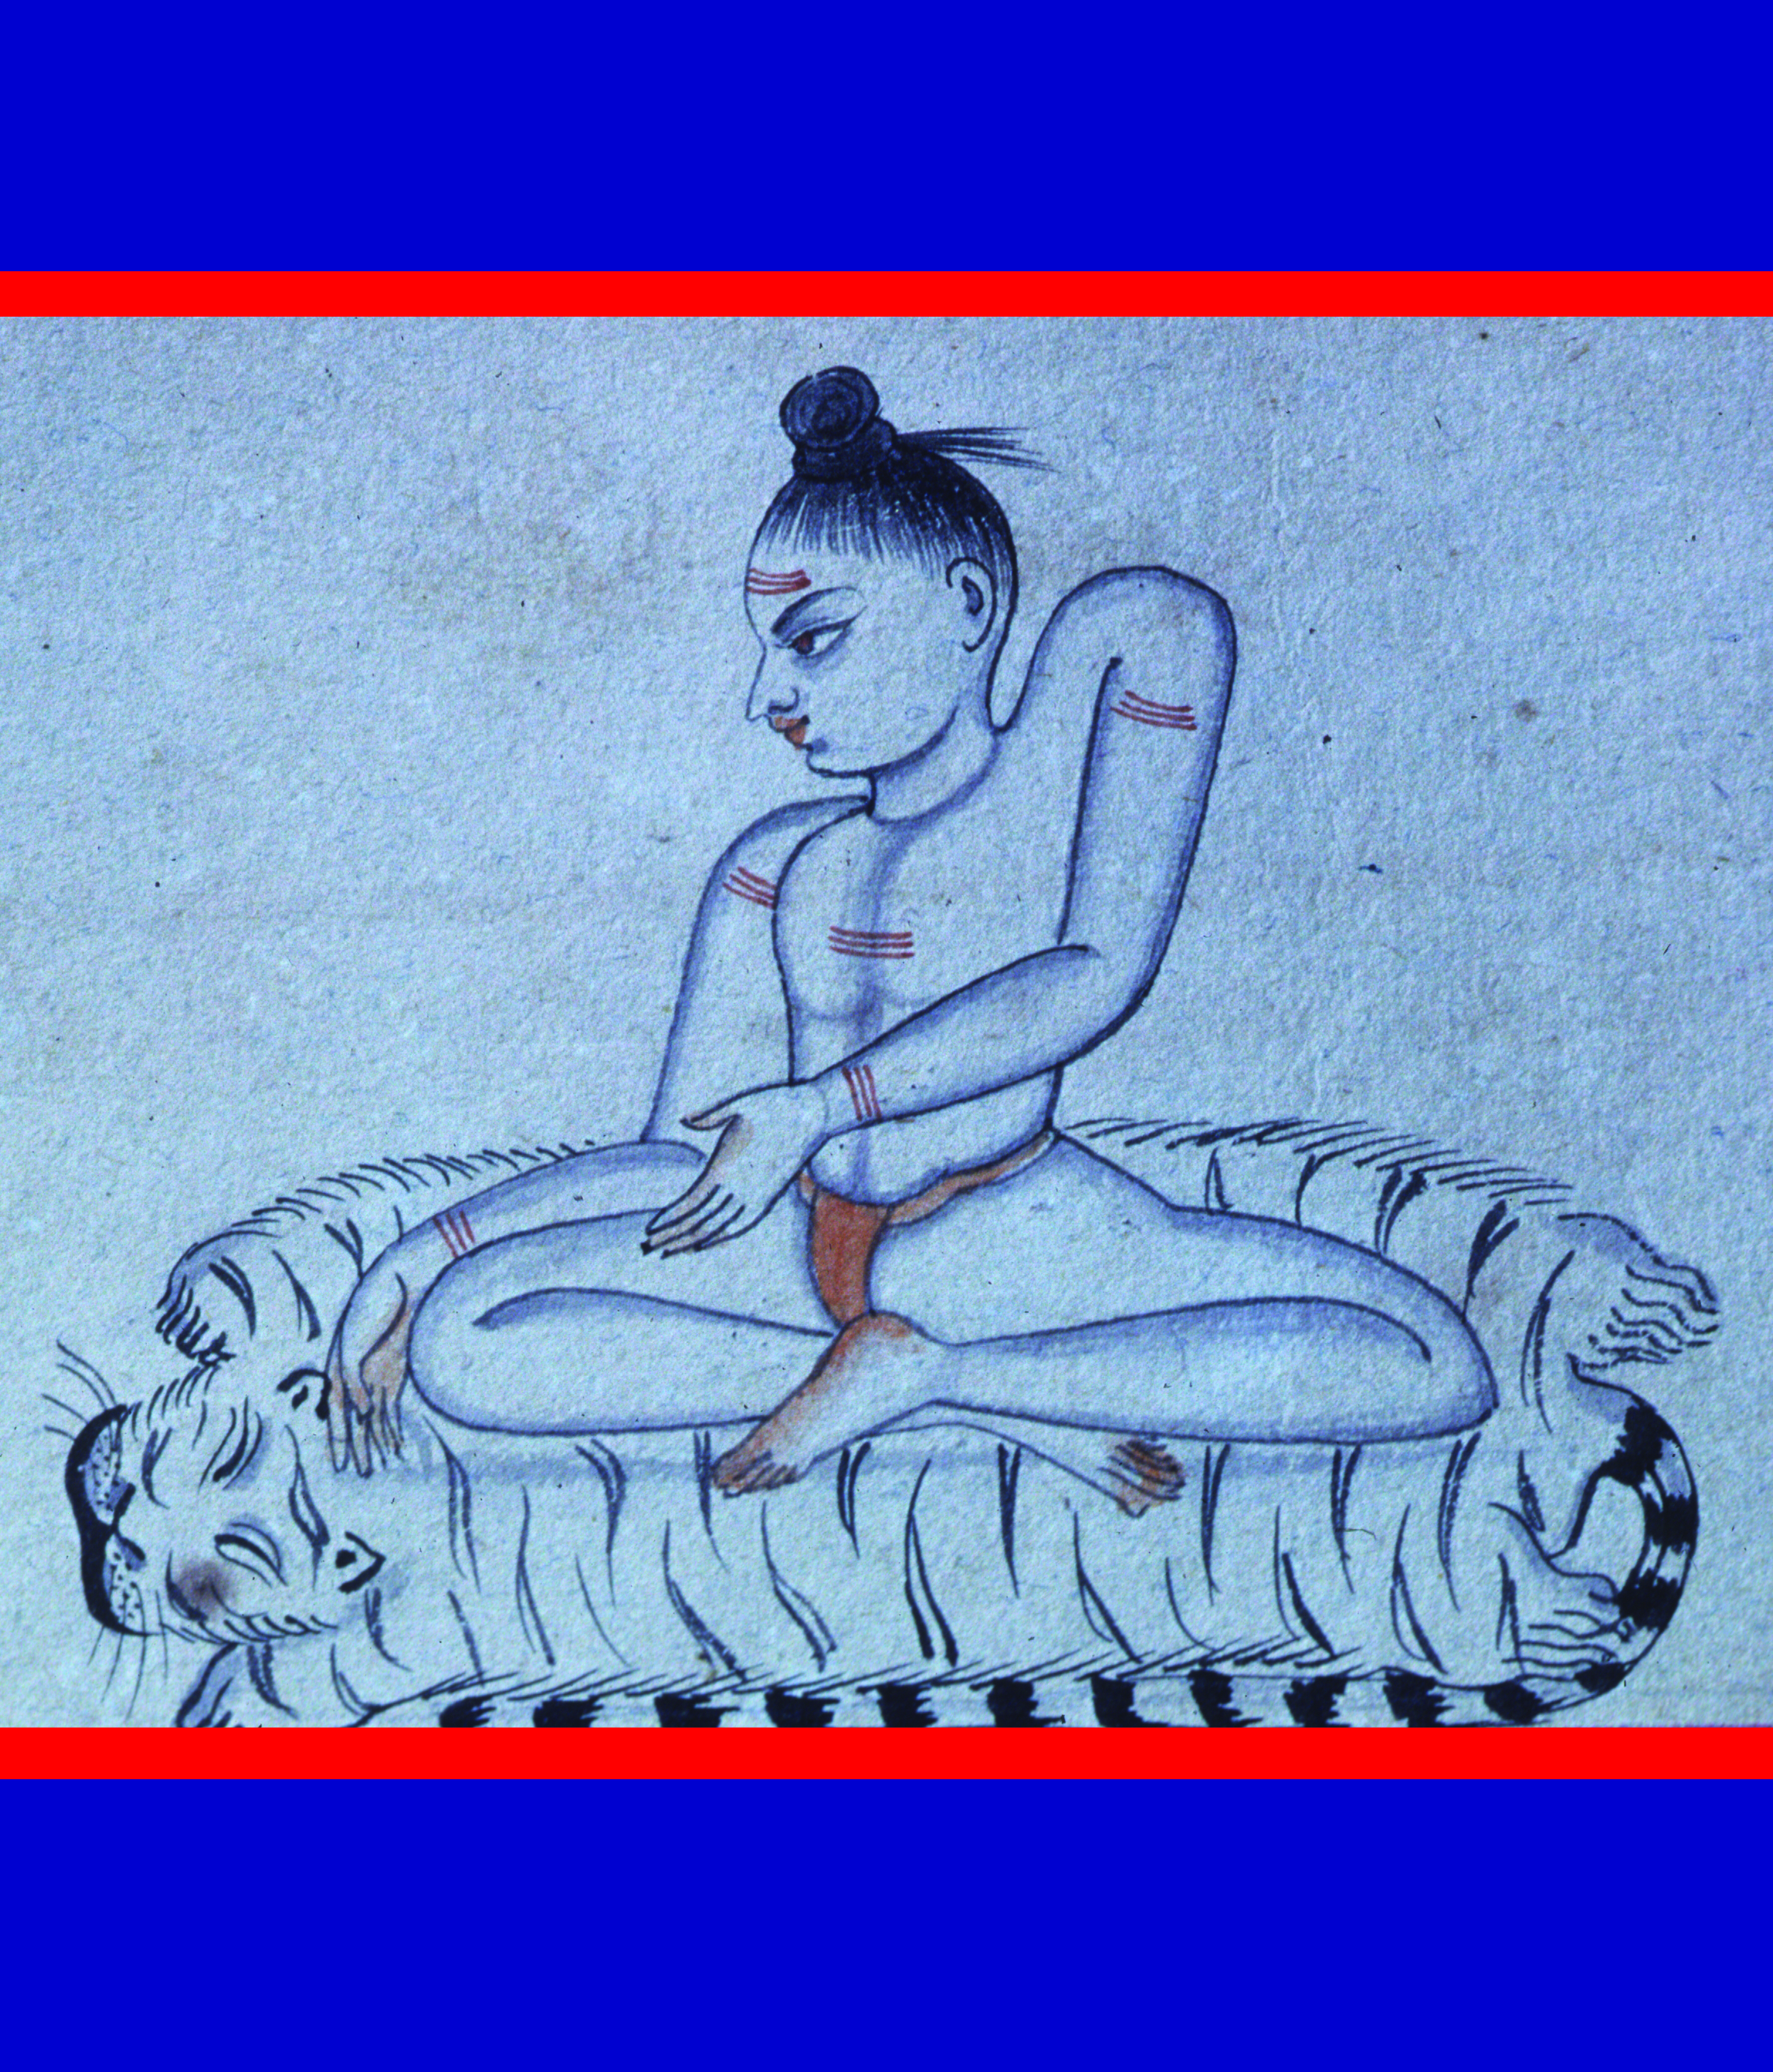
\includegraphics[width=\paperwidth, height=\paperheight, keepaspectratio]{2.jpg}
  %};
%\end{tikzpicture}

%\newpage

\input src/sample

\newpage

~\vskip 1cm

\begin{multicols}{2}
\thispagestyle{empty}
\theendnotes
\end{multicols}
\end{document}
